\documentclass[table,15pt,t]{beamer}

\usepackage{fontspec}
\usepackage{xunicode} %Unicode extras!
\usepackage{xltxtra}  %Fixes
\usepackage{relsize}  %relative font sizing commands
\usepackage{booktabs}
\usepackage{eulervm} %mathfonts
\usepackage{tikz}
\usepackage{listings}
\usepackage{graphicx}
\usepackage{tabularx}
\usepackage{alltt}
\usepackage{ifthen,calc}

\usetheme{Sleek}

\usetikzlibrary{arrows,shapes,shadows}
\usetikzlibrary{positioning}

\tikzstyle{ds} = [draw, thick, color=oxygenblue, inner sep=0pt, drop shadow]

\setsansfont[Mapping=tex-text]{Trade Gothic LT Std}

\setlength{\fboxsep}{2mm}
\newcommand{\sem}[1]{\ensuremath{[\![#1]\!]}}

\title{Optimized Translation of Clafer Models to Alloy}
\author{Kacper Bak}
\institute{\small Generative Software Development Lab\\University of Waterloo}
\date{CS744 Course Project. July 19, 2011}

\newcommand{\vmiddle}[1]{
  \vspace{\stretch{1}}
  #1
  \vspace{\stretch{1}}
}

\newcommand{\interframe}[1]{
\begin{frame}{}
\vmiddle{\hmiddle{\Huge #1}}
\end{frame}
}

\newcommand{\mlist}[1]{
\vmiddle{
  \begin{list}{}{}
    #1
  \end{list}
  }
}

\newcommand{\hmiddle}[1]{
  \begin{center}#1\end{center}
}

\newcommand{\twocolumns}[4]{
    \begin{columns}
      \begin{column}{#1\textwidth}
        \begin{overlayarea}{#1\textwidth}{\textheight}
          #2
        \end{overlayarea}
      \end{column}
      \begin{column}{#3\textwidth}
        \begin{overlayarea}{#3\textwidth}{\textheight}
          #4
        \end{overlayarea}
      \end{column}
    \end{columns}
}

\newcounter{i}
\newcommand{\ganimate}[3]{
    \setcounter{i}{0}
    \whiledo{\value{i}<#2}{
      \stepcounter{i}
      \only<\the\value{i}>{\includegraphics[#3]{figs/#1\the\value{i}}}
    }
}

\newcommand{\showCode}[3]{
  \only<#1>{\lstinputlisting[firstline=#2,lastline=#3]{code/telematics.cfr}}
}

\makeatletter
\newcommand{\showCodesStart}[3]{
\setcounter{i}{#1}
\@for\arg:=#3\do{
  \showCode{\value{i}}{#2}{\arg}
\stepcounter{i}
}}
\makeatother

\newcommand{\showCodes}[2]{
\showCodesStart{1}{#1}{#2}
}

% To make the legend for icons in class diagrams
\newcommand{\icon}[1]{\textcircled{\texttt{\textbf{\textit{#1}}}}}

\lstdefinelanguage{Clafer}
{morekeywords={abstract, else, in, no, opt, xor, all, enum, lone, not, or, disj, extends, mux, one, some},
sensitive=true,
morecomment=[l][\footnotesize\itshape]{--},
morecomment=[s][\small\itshape]{{-}{-}},
%basicstyle=\footnotesize,
tabsize=4,
columns=fullflexible,
literate={->}{{$\to$ }}1 {^}{{$\mspace{-3mu}\widehat{\quad}\mspace{-3mu}$}}1
 {<}{$<$ }2 {>}{$>$ }2 {>=}{$\geq$ }2 {<=}{$\leq$ }2
 {<:}{{$<\mspace{-3mu}:$}}2 {:>}{{$:\mspace{-3mu}>$}}2
 {<=>}{{$\Leftrightarrow$ }}2
 {=>}{{$\Rightarrow$ }}2 {+}{$+$ }2 {++}{{$+\mspace{-8mu}+$ }}2
 {\~}{{$\mspace{-3mu}\widetilde{\quad}\mspace{-3mu}$}}1
 {!=}{$\neq$ }2 {*}{${}^{\ast}$}1
 {\#}{$\#$}1
 {\~}{$\neg$}1
 {+}{$+$ }1
}

\lstset{basicstyle=\small,language=Clafer,numbers=none}

\begin{document}

\begin{frame}[plain]
  \vmiddle{\titlepage}
\end{frame}

\begin{frame}{Course Project}
  \mlist{
  \item CS 744: Advanced Compiler Design
  \item Data flow analysis, redundancy elimination, optimizations
  \item Individual project
  \item Duration: 2 months
  }
\end{frame}

\begin{frame}{Clafer Update}
  \mlist{
    \item Analysis of variability models
    \item Translation to Alloy (uses SAT solvers)
    \item \textsf{clafer2alloy} translator: a year ago
    \item Some work on formal semantics
    \item Examples of variability models
  }
\end{frame}

\begin{frame}{The Toolchain}
  \begin{tabularx}{\textwidth}{ccccccccc}
    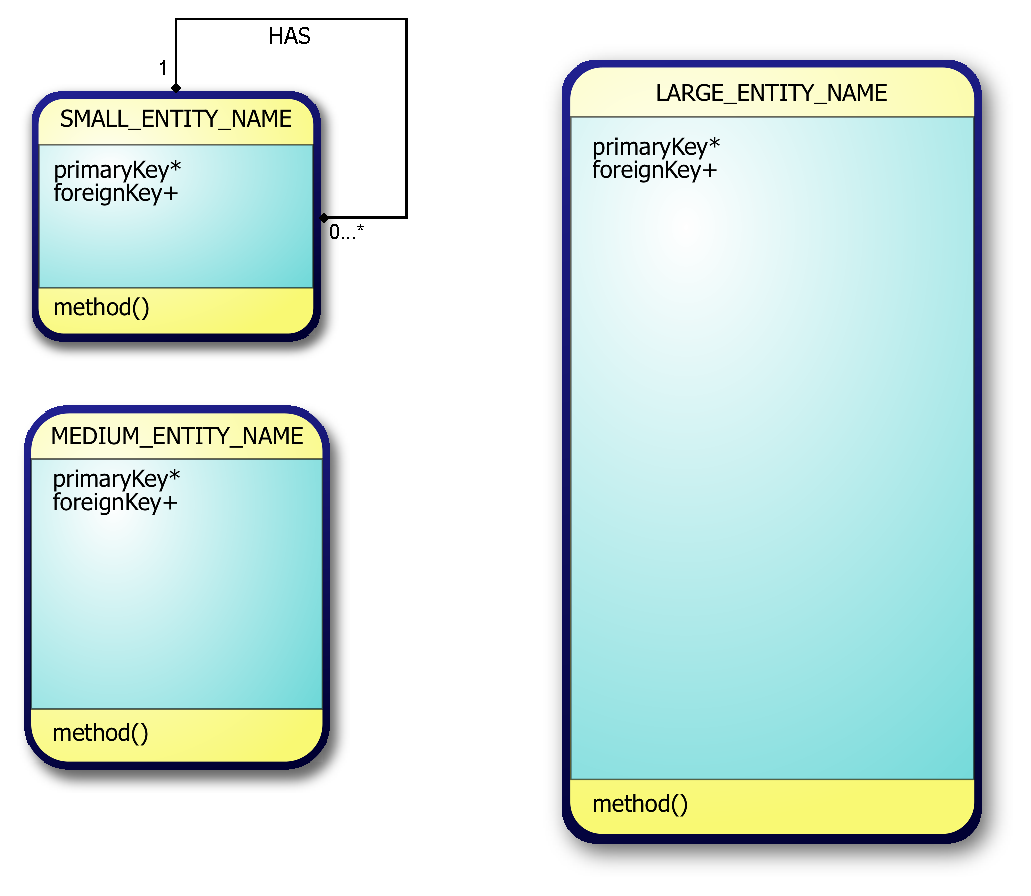
\includegraphics[scale=0.06]{figs/model}
    & $\rightarrow$
    & 
\includegraphics[scale=1]{figs/gears}
    & $\rightarrow$
    & 
\includegraphics[scale=0.3]{figs/document}
    & $\rightarrow$
    & 
\includegraphics[scale=0.7]{figs/alloy}
    & $\rightarrow$
    & $P \land Q$
    \\
    Clafer & & Clafer & & Alloy & & Alloy & & Formula\\
    Model & & Translator & & Model & & Analyzer & &
  \end{tabularx}
\end{frame}

\interframe{Demo}

\begin{frame}{Problems}
  \begin{tabularx}{\textwidth}{ccccccccc}
    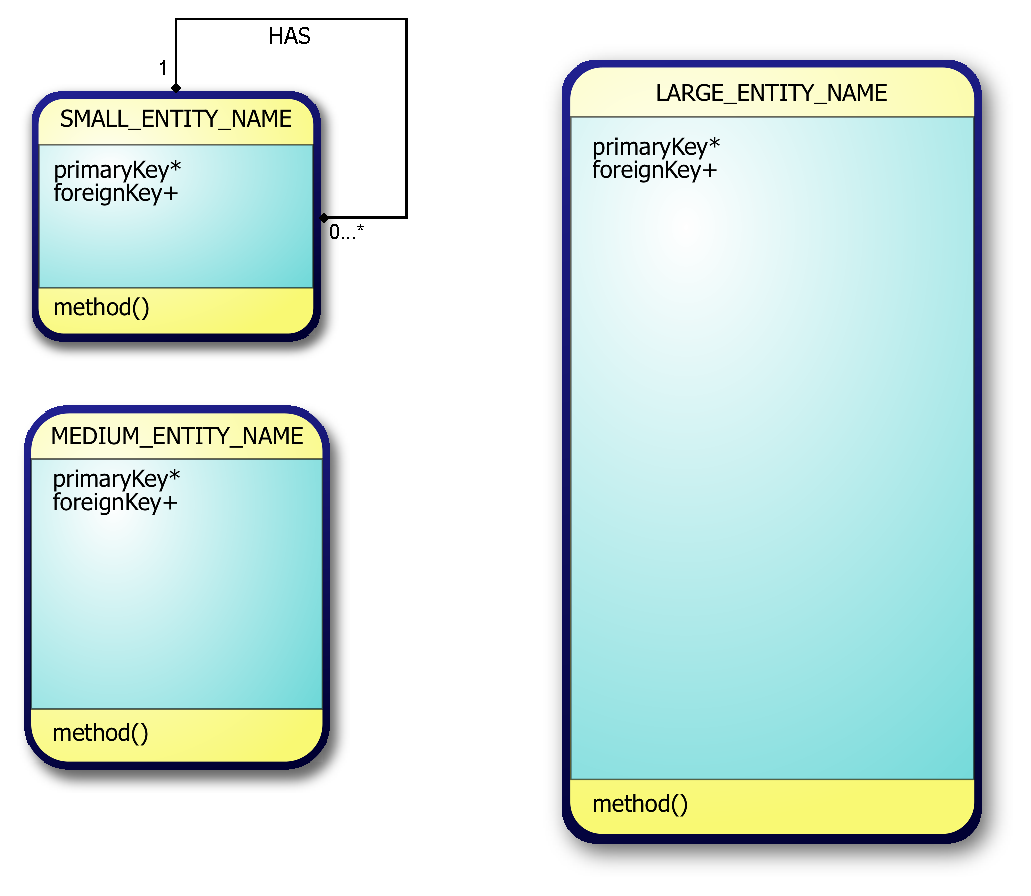
\includegraphics[scale=0.06]{figs/model}
    & $\rightarrow$
    & 
\includegraphics[scale=1]{figs/gears}
    & $\rightarrow$
    & 
\includegraphics[scale=0.3]{figs/document}
    & $\rightarrow$
    & 
\includegraphics[scale=0.7]{figs/alloy}
    & $\rightarrow$
    & $P \land Q$
    \\
    Clafer & & Clafer & & Alloy & & Alloy & & Formula\\
    Model & & Translator & & Model & & Analyzer & &
  \end{tabularx}
  \mlist{
  \item \visible<1->{Translation rules heavily influence reasoning time in Alloy}% bottlenecks
  \item \visible<2->{Large Alloy files (complex models)}
  \item \visible<3->{Ineffective Alloy representation (complex formulas)}
  \item \visible<4->{Slow \textsf{clafer2alloy} translator}
 }
  \begin{tikzpicture}[overlay]
    \draw<2->[red,ultra thick,rounded corners] (5.0,4.0) rectangle (7.0,7.0);
    \draw<3->[red,ultra thick,rounded corners] (10.0,4.0) rectangle (11.75,7.0);
    \draw<4->[red,ultra thick,rounded corners] (2.3,4.0) rectangle (4.3,7.0);
  \end{tikzpicture}
\end{frame}

\begin{frame}{Solution}
 \mlist{
    \item Refactored and modular code architecture
    \item User has control over the translation process
    \item Intermediate language representation
    \item Optimization of translation rules 
 }
\end{frame}

\interframe{The Translator}

\begin{frame}{(Old) clafer2alloy Translator}
 \mlist{
    \item Parser, desugarer, semantic analyzer, code generator
    \item Monolithic
    \item Haskell
    \item Available online
    \item Released source code
 }
\end{frame}

\begin{frame}{(New) clafer Translator}
 \mlist{
    \item Front-end, intermediate representation, optimizer, generators
    \item User can turn on/off modules (has extra knowledge)
    \item Easy to add new code generators
 }
\end{frame}

\interframe{Optimizations}

\begin{frame}[fragile]
  \frametitle{No Unused Abstract Clafers}
  \begin{columns}
    \begin{column}{0.5\textwidth}
      \begin{alltt}
        \begin{small}
\textbf{abstract} \textsf{display}
  \textsf{server} ?

\textsf{OnBoardComputer}
        \end{small}
      \end{alltt}
    \end{column}
\pause
    \begin{column}{0.5\textwidth}
      \begin{alltt}
        \begin{small}
\textsf{OnBoardComputer}
        \end{small}
      \end{alltt}
    \end{column}
  \end{columns}
\end{frame}

\begin{frame}{No Redundant Hierarchical Constraints} %parent
\textsf{ElectronicControlUnit} 2
  \textsf{display} 1..2

\end{frame}

\begin{frame}{Improved Name Resolution}
% elements have unique names -> fewer constraints
\end{frame}

\begin{frame}{Global Cardinality Constraints}

\end{frame}

\begin{frame}{Integers as Attributes} %not refs

\end{frame}

\begin{frame}{References are Relations} %no extra constraints

\end{frame}

\begin{frame}{Unrolled Inheritance}

\end{frame}

\begin{frame}{Model Statistics}

\end{frame}

\interframe{Evaluation}

\interframe{Conclusion}

\begin{frame}{Conclusion}
 \mlist{
    \item Modeling and analyzing SPLs\pause
    \item Concept modeling\pause
    \item Common infrastructure\pause
    \item Non-trivial analyses
 }
\end{frame}

\interframe{Thanks for listening!}

\interframe{Questions?\\[1cm]\normalsize{\textsf{gsd.uwaterloo.ca/clafer}}}

\end{document}
